\documentclass[11pt,french,english]{article}
\usepackage[T1]{fontenc}
\usepackage[utf8]{inputenc}
\usepackage{amssymb}
\usepackage{mathtools}
\usepackage{bbm}
\usepackage{ulem}
\usepackage{url}
\usepackage{graphicx}
 \usepackage{geometry}
\geometry{margin=1.0in}

\usepackage{lmodern}
\usepackage[english]{babel}
\makeatletter
\addto\extrasfrench{%
   \providecommand{\og}{\leavevmode\flqq~}%
   \providecommand{\fg}{\ifdim\lastskip>\z@\unskip\fi~\frqq}%
}
\makeatother

\usepackage{etoolbox}


%%%%%%%%% STUDENTS CHANGE THIS

\providetoggle{undergrad}
\settoggle{undergrad}{false}     %%% "true" if 3395 or "false" if 6390

\providetoggle{french}
\settoggle{french}{false}        %%% "true" if french or "false" if english

\providetoggle{final}            
\settoggle{final}{false}        %%% "true" for your final homework submission (removes instructions)

%%%%%%%%%%%%%%%%%%%%% ^^^^^
\usepackage[colorlinks=true]{hyperref}


\begin{document}

\setlength{\parskip}{0.3cm} \setlength{\parindent}{0cm}

\begin{center}
\textbf{\proftitle{IFT 6390 Fundamentals of Machine Learning \\ Vijaya lakshmi Kuruba\\ Saadaoui Houda}}
\par\end{center}{\large \par}

\begin{center}
\textbf{\LARGE{\enfr{Model Card - SVM Linear Classifier}}}
\par\end{center}{\LARGE \par}

Our model is a supervised learning which consists of classifying gender using tweets and users profile description. 
Since it is a supervised learning task we used a dataset consisting of tweets labeled with the gender “male” or “female”.

The dataset used has 20,000 samples and has many features but to build our model we chose only two features: tweets and description.

Before building our model, we first cleaned the data using the following steps:
\begin{itemize}
    \item Choosing only the gender "female" and "male" (the data has also unknown and brand as genders)
    \item Preprocessing the data using the Preprocessor library
\end{itemize}

After filetring and preprocessing the dataset, we ended up with 12,895 samples which we split into training and testing with 80\% and 20\% respectively of the dataset.  \\
We chose to use the linear classifier Support Vector Machine SVM to make the classification task.

Model parameter is validated with K fold cross validation and classifier metrics has been reported.

\paragraph{SVM Linear Classifier}: 

$$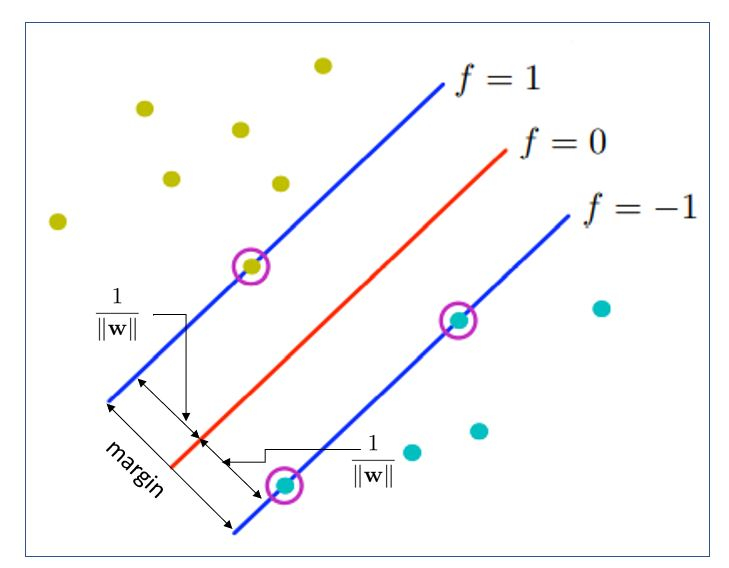
\includegraphics[scale=.5]{svm.JPG}$$

We consider labeled data $(\mathbf{x},y)$, where $\mathbf{x}$ is a $d$-dimensional input, i.e. $\mathbf{x} \in \mathbb{R}^{d}$ and $y\in\{-1,1\}$. We have a dataset of $n$ such pairs $(\mathbf{x}_i,y_i)$. We want to train a linear classifier on this dataset. \\

\textbf{Linear Model:}
\begin{equation}
 f(x) = \mathbf{w}^T \mathbf{x} + b   
\end{equation}
On Hyper plane :
\begin{equation}
f(x) =\mathbf{w}^T \mathbf{x} + b=0    
\end{equation}
Constraints are:
\begin{equation}
 \mathbf{w}^T \mathbf{x_i} + b\geq 1 \quad \text{if} \quad y_i=1 
 \end{equation}
\begin{equation}
 \mathbf{w}^T \mathbf{x_i} + b\leq -1 \quad \text{if} \quad y_i=-1   
\end{equation}

In general 
\begin{equation}
    y_i(\mathbf{w}^T \mathbf{x_i} + b)\geq 1 \quad \forall \quad i \in 1...N 
\end{equation}


To simplify code and notation, we can get rid of the bias term $b$. To do  so, we concatenate $1$ to every $\mathbf{x}$ vector, so that $\mathbf{x}' = (\mathbf{x}, 1) \in \mathbb{R}^{d+1}$, and we concatenate $b$ to $\mathbf{w}$, so that $\mathbf{w}' = (\mathbf{w}, b)$. Then $\mathbf{w}^T \mathbf{x} + b = \mathbf{w}'^T \mathbf{x}'$. We can write everything in terms of linear transformations instead of affine transformations.

We will omit the bias term from now on, and consider $\mathbf{x}$ and $\mathbf{w}$ themselves as $\mathbf{x}'$ and $\mathbf{w}'$

New notation: 
\begin{align}
    y_i(\mathbf{w}^T \mathbf{x_i} )\geq 1 \quad \forall \quad i \in 1...N    
\end{align}

\textbf{Loss Function :} \\
\\The hinge loss is used for "maximum-margin" classification.\\
Loss function is given by:

\begin{equation}
 g(w;\mathbf{x}, y)  
& =
\begin{cases}
0 \quad \quad \quad \quad\quad \text{if}\quad 1-yf(x) \geq 1 \\ 1-yf(x) \quad\text{otherwise.}
\end{cases}
\end{equation}


\textbf{Objective Function:}\\
 \\The loss function stated above is called convex surrogate losses. They are convex and have a gradient so we can optimize them with gradient descent.\\
 
The training objective that we are going to minimize is the average of the losses over each training example plus an $\ell^2$ regularization with hyperparameter $\lambda$:
\begin{align}
 L(w) = \frac{1}{n}\sum_{i=1}^n g(w;\mathbf{x_i}, y_i)  + \frac{\lambda}{2} \| \mathbf{w}\|^2   
\end{align}

Note:  Minimising w allows to maximize the margen

where the parameter $\lambda$  determines the trade-off between increasing the margin size and ensuring that the $\mathbf {x} _{i}$ lie on the correct side of the margin. Thus, for sufficiently small values of $\lambda$ , the second term in the loss function will become negligible, hence, it will behave similar to the hard-margin SVM, if the input data are linearly classifiable, but will still learn if a classification rule is viable or not.

\textbf{Gradient Desecent:}  

SVM classifier amounts to minimizing the loss funtion Equation 8 with Gradient descent technique.
We want to minimize the loss $L(w)$. It is differentiable, so we can use the gradient descent algorithm: start from any initialization parameter $\mathbf{w}_0$, and repeat for $t\in\{0, \dots, t_\max \}$:
$$\mathbf{w}_{t+1} = \mathbf{w}_t - \eta\ \nabla L (\mathbf{w}_t) \; .$$

Under some conditions on the step-size $\eta$ and the loss $L$, this algorithm is guaranteed to converge to a minimum of $L(w)$.

$$\nabla L (\mathbf{w}_t)=\lambda \| \mathbf{w}\| \quad \text{if} \quad 1-yf(x)\geq 1$$
$$$$

$$\nabla L (\mathbf{w}_t)
=
\begin{cases}
\lambda \| \mathbf{w}\| \quad \quad \quad \quad\quad \text{if}\quad 1-yf(x) \geq 1 \\ \lambda \| \mathbf{w}\|-y_ix_i \quad\text{otherwise.}
\end{cases}
$$

To choose the $\lambda $ parameter, we used a Randomized Search to get the best value among the following list [1e-4, 1e-3, 1e-2, 1e-1, 1e0, 1e1, 1e2, 1e3]. The obtained value of $\lambda $ is 0.001

\paragraph{K fold Crossvalidation}: 

To evaluate the performance of a model on a dataset, we need to measure how well the predictions made by the model match the observed data. 
When data is scarce, we may not be able to afford using a validation set, So we use K fold crossvalidation technique.\\
Approach : split the dataset into K equal partitions.
\begin{itemize}
    1. Set one partition aside for prediction/validation, and train the model on the remaining K-1 partitions.\\
2. Repeat the above step for each partition and report the average prediction error.

\end{itemize}

In pratice: common to pick 5-fold or 10-fold cross-validation.

Mathematically: 
$$
        CV(\hat{f}) \defeq= \frac{1}{N} \sum_{i=1}^N L(y_i, \hat{f}^{(\kappa(i))}(x_i)) \enspace $$
where $\hat{f}(k)$ denotes the model obtained by removing the k-th partition and training on the
rest. Furthermore, k(i) is a function which, given a datapoint index, returns the partition to
which it belongs. If the i-th datapoint belongs to the j-th partion, then we want the model
$f^{(j)}$
, where the j-th partition has been excluded.


For our model, after cleaning and filtering the data we used K-Folds Cross Validation technique using k = 5 to validate it.

\paragraph{Classifier Accuracy }: 
\begin{align*}
    Accuracy (y, \hat{y})= \frac{1}{N} \sum_{i=1}^N \mathbbm{1}_{\hat{y_i} = y}
\end{align*}
where $\mathbbm{1} (x)$  is the indicator function.

\\
\paragraph{Time Complexity}:

N= Number of training examples\\
k=k is the number of iterations (epochs)\\ 
d=Dimensions of the features

Time complexity for training is : O(Nkd)

Time complexity for testing is : O(Nd)

\\
\paragraph{Space Complexity}:

N= Number of training examples\\
d=Dimensions of the features

Space complexity for training is : O(kd)

Space complexity for testing is : O(Nd)
\end{document}
